\documentclass[11pt]{article}

\usepackage[margin = 1 in]{geometry}
\usepackage[pdftex]{graphicx}
\graphicspath{{images/}}
\usepackage{subfigure}
\usepackage{booktabs}
\usepackage{multirow}
\usepackage[table]{xcolor}
\usepackage{array}
%\usepackage{amsmath}
\usepackage{booktabs}
\usepackage{multirow}
\usepackage{amsmath}
\usepackage{url}
\renewcommand\UrlFont{\color{blue}}
\usepackage[colorlinks=true,urlcolor=blue]{hyperref}

\title{Project Report Team 03\\
Integrated Map of Risk Information in Colombia}
\author{ Johnathan Salamanca, Mario Cer\'{o}n, \\
Carol Martinez, Javier Cocunubo, Jairo Ni\~no, Alvaro Mu\~noz
 }
\date{\today}

\begin{document}
\maketitle

%\begin{abstract}

%In this document \ldots
%\end{abstract}


\section{Introduction}
\label{sec:Intro}
Introduction section of final report written.
This should clearly state the context of your team?s application and the problem you set out to solve, as well as your justification for why it is an important problem.




%Table \ref{tabDataset} summarizes the information of the datasets.
%
%\begin{table}[h]
%\begin{center}
%\label{tabDataset}
%\begin{tabular}{|c|c|c|c|c|}
%\hline
%\textbf{Data Name} & \textbf{Description} & \textbf{Type} & \textbf{Number} & \textbf{Database}   \\
%\hline
% Event name: & type of disaster (flooding,XX)& categorical &S &  UNGRD\\
% Date: & incident date & numerical &XXX &  UNGRD/DANE  \\
% Code: &disaster ID & numerical &XXX &  UNGRD/DANE  \\
% Municipality Code: & Divipola code & numerical &XXX &  UNGRD/DANE  \\
% Dead: & Deads per incident & numerical &XXX &  UNGRD  \\
% Wounded: & Wound per incident & numerical &XXX &  UNGRD  \\
% Disappeared: & Disappeared per incident & numerical &XXX &  UNGRD  \\
%  Affected: & Affected people & numerical &XXX &  UNGRD  \\
%   Affected families: & Affected people & numerical &XXX &  UNGRD  \\
%\hline
%\end{tabular}
% \caption{Summary of the main information available to develop the project.}
%\end{center}
%\end{table}
%



%  (data of ):
%http://portal.gestiondelriesgo.gov.co/Paginas/Consolidado-Atencion-de-Emergencias.aspx
%We plan to cross data from the previous dataset with data from the DANE, IDEAM
%We may require datasets to extract data of:
%Hospitals available in the area
%Schools
%Emergency services available.
%Demographic data



%Santos talks about Colombia Progress on Risk Management https://www.unisdr.org/archive/58870

%? ?El Ni�o? and particularly the La Ni�a 2010-2011, which generated a national emergency situation never before seen in the country, affecting nearly 765 municipalities in Colombia, ?. After these phenomena, the government decided to improve the gathering information systems (info taken from
%https://library.wmo.int/doc_num.php?explnum_id=4759 )


%\section{Project scoping plan/proposal written}
%\label{sec:app}

%\subsection{Project scope}
%
%\begin{itemize}
%\item The Government Officials (at all levels) are our main stakeholders
%\item Boundaries of the project:
%\begin{itemize}
%\item We do not offer forecasts or modeling/ infer data.
%\item We only show metrics of impact of disasters at municipal level (not pin point to specific disaster event)
%\item We do not offer recommendations, only do support to decision making process for the stakeholders.
%\end{itemize}
%\item Risks
%\begin{itemize}
%\item Data quality issues in the datasets 
%\item The available data might be not enough to solve the proposed problem.
%\end{itemize}
%\end{itemize}


%\subsection{Project plan}

%\textbf{Problem}: The Municipal Capacities’-Adjusted Disaster Risk Index is an innovative indicator for policymakers to make informed decisions about how to better preserve citizens’ well-being in the presence of real and potential threats.
%However, to be actionable, information needs not only to be available but efficiently delivered to communities. As a means of protecting citizen’s rights, foster economic growth, and make government officials accountable.
%As per its current state, official risk management information lacks a delivery system that enables local communities to improve their risk awareness and disaster coping capabilities in different scenarios marked for global phenomena such as extreme temperatures and changing weather patterns.
%For instance, it is not apparent how similar events have impacted communities with different risk and vulnerability profiles, relevant information to assess the performance of risk management activities.

 %Impact is defined in terms of: Inhabitants affected/Thousand Inhabitants, percentage of households affected, Deceased/ Thousand Inhabitants.\\

%\begin{itemize}
%\item \textbf{Expected Deliverable}:\\
%To cope with the challenges stated before, our approach includes a dynamic map of Colombia delivering:
%
%\begin{enumerate}
%\item The impact metric (or metrics) at the municipal level for a given category of events. Ability to display complementary metrics of interest for specific locations (utilities, healthcare facilities, first-responder facilities, etc).
%\item Considering the established association between extreme temperatures and the frequency of hydro-meteorological events, a projected extreme-temperature indicator for the 100 most vulnerable municipalities with 3 data points: Indicator value at Time 0 (1998), Time 1 (2018) and Time 3 (projected 2040)
%\item The indicator corresponds to the extreme temperature projection made by Climate Impact Lab for the number of days a year that register temperatures above 32 degrees Celsius.
%\end{enumerate}


%
%
%\item \textbf{How do we get there?}:
%
%\begin{itemize}
%\item Get datasets, clean, wrangled, and analyze them.
%\item Data modeling
%\item Load the data in the cloud (RDS on AWS) and the instance (EC2) for hosting the back and front ends. Install and review the environment.
%\item Make the back end: review databases, environment and set the code for running in the cloud
%\item Make the front end : Interactive Colombian Map in Dash and tested on AWS.
%\item Make the final presentation
%\item Make the final report
%\end{itemize}
%
%\end{itemize}
%
\section{Application Overview}
\label{sec:appOver}


\subsection{Users}
Any person, Government officials, or someone in the private sector who wants to read and understand the basic risk profile of their region and make decisions with that information.

\subsection{Architecture}

Figure \ref{fig:archi} shows the architecture of the proposed solution including the elements of the application at component level and its connections at high level (see deployment diagram). Additionally, it shows the application elements used for the Front and Back End. The figure also shows the names of the technologies used hosted on AWS cloud, i.e.: (Python, dash and libraries).   

The following is the list AWS components used in the project: 
\begin{enumerate}
\item The machine who host the solution (Elastic Compute Cloud - EC2). 
\item The Database  (Relational Database Service -RDS).
\item The storage for the datasets and GeoJson files for Colombia on the service  (Simple Storage Service - S3) to save these files.
\item The Security group for these services talks with each other and have access from the internet as well.
\item The remote DNS (Domain Name Service) to have a friendly URL for the application on the Apache Web server.
\item A remote code repository (hosted by github). It is used for hosting the source code and documentation. 

\end{enumerate}


\begin{figure}%
\centering
\subfigure[Deployment diagram]{%
\label{fig:first}%
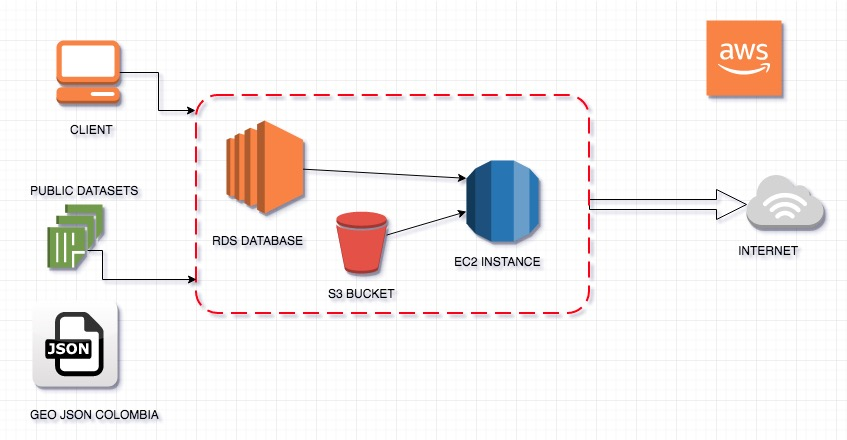
\includegraphics[height=3in, width=4.5in]{../../../aws_diagrams/AWS_Deployment_Diagram_project_group_03}}%
\qquad
\subfigure[Component diagram]{%
\label{fig:second}%
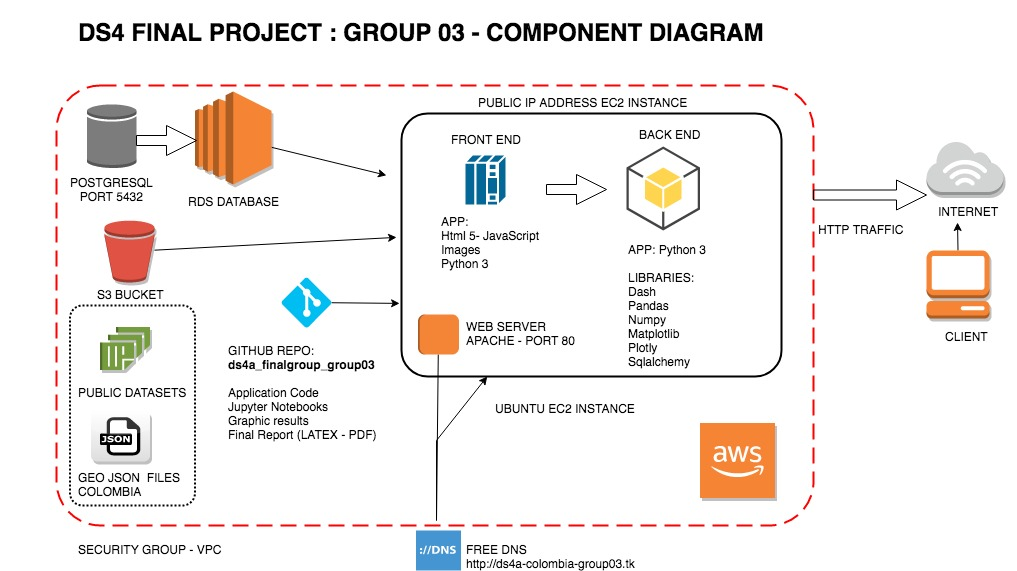
\includegraphics[height=4in, width=6in]{../../../aws_diagrams/AWS_Component_Diagram_project_group_03}}%
\caption{Project architecture.}
\label{fig:archi}%
\end{figure}





\subsection{Front End Design}

The following is the link of the web-page created for the project. \\
 \url{http://ds4a-colombia-group03.tk/}
%\item \href{https://marioceron-case-51.s3.amazonaws.com/final_project/front_end/index.html}{http://ds4a-colombia-group03.tk/} 

In general terms, the proposed information system will provide a dynamic map of Colombia with:

\begin{enumerate}
\item Impact variables such as Deaths, People and Houses affected.
\item A map (Main View) that will show the index adjusted by capacity ( \'Indice Ajustado por Capacidades). By default, the map starts with the country view with political division (departamento).
\item A timeline slider will facilitate the visualization of the index using time intervals. 
\item Considering the established association between extreme temperatures and the frequency of hydro-meteorological events, a projected extreme-temperature indicator for the 100 most vulnerable municipalities with 3 data points: Indicator value at Time 0 (1998), Time 1 (2018) and Time 3 (projected 2040). The indicator corresponds to the extreme temperature projection made by Climate Impact Lab for the number of days a year that register temperatures above 32 degrees Celsius.

\item The option of showing political divisions views (vista de departamento). The user can select the small political subdivision (municipio) and the graphics on the right side of the dashboard screen are updated.
\end{enumerate}




\begin{figure}%
\centering
\subfigure[Presentation page]{%
\label{fig:first}%
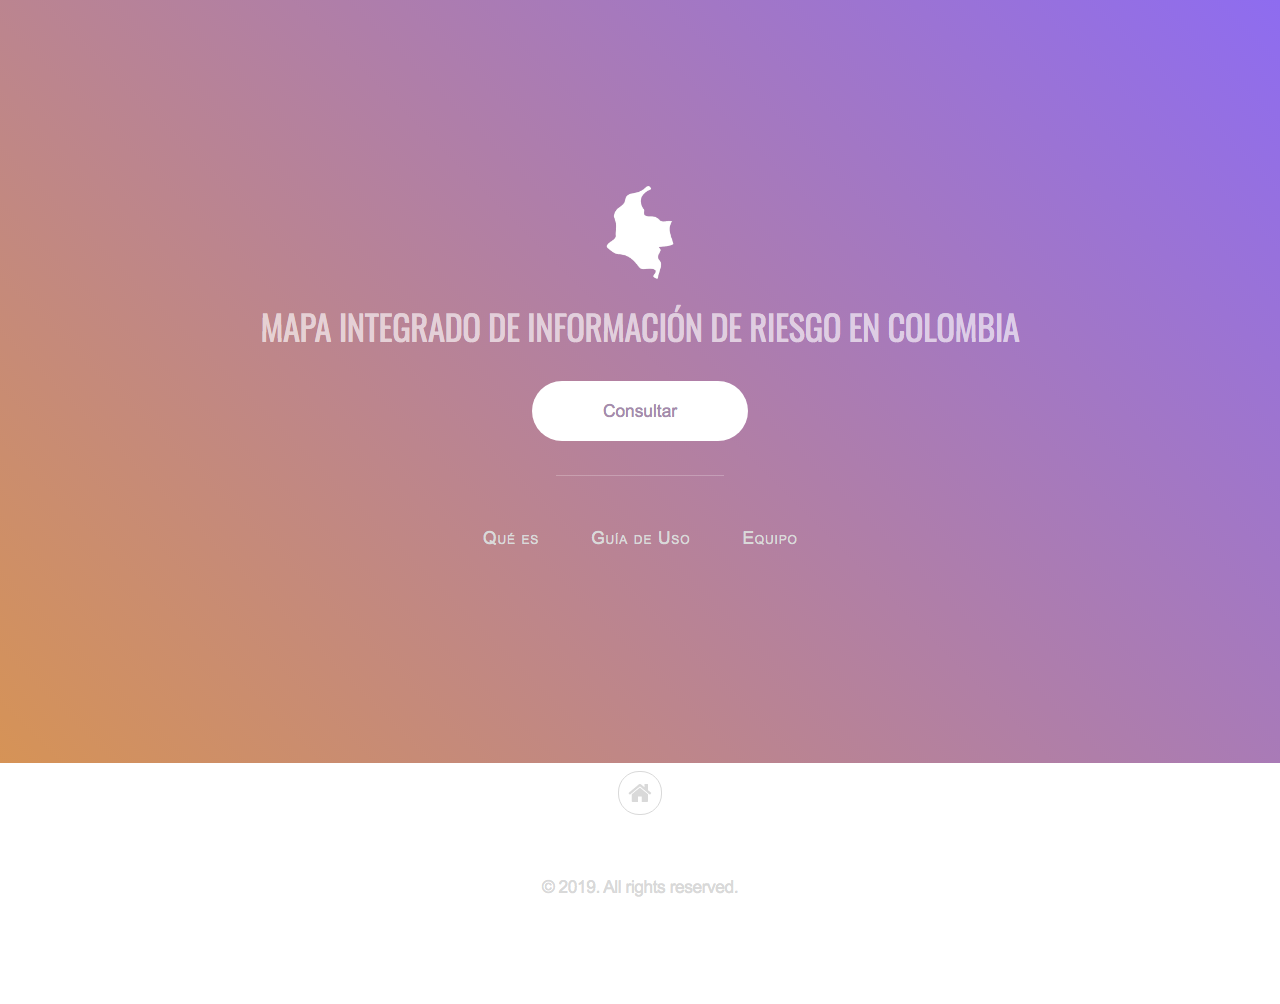
\includegraphics[height=4in, width=6in]{01_Home_ds4a-colombia-group03-tk.png}}%
\qquad
\subfigure[Main page]{%
\label{fig:second}%
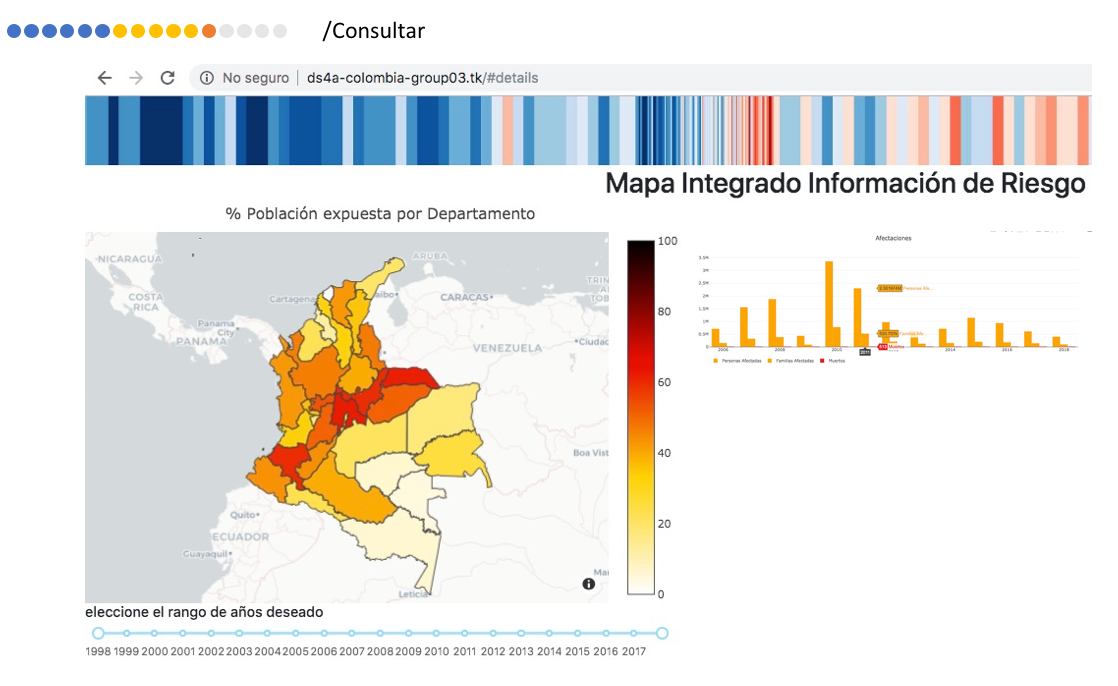
\includegraphics[height=4in, width=6in]{02_Home_mapa.png}}%
%\subfigure[]{%
%\label{fig:second}%
%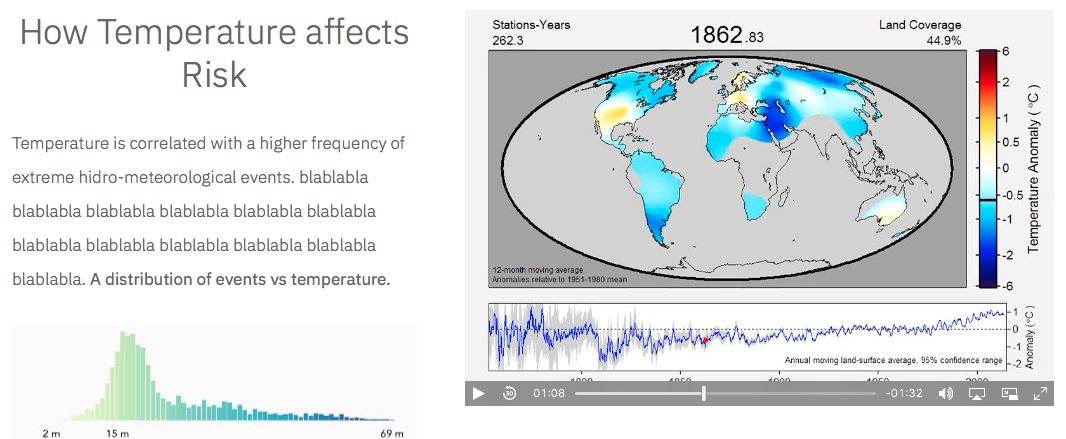
\includegraphics[height=2in, width=3in]{riesgo6}}%
\caption{Front End: Integrated Map of Risk Information in Colombia. The main page (Figure \ref{fig:first}) will show the map of Colombia with the Risk Index, and will offer interactive options to get detail information of selected Municipalities, risk index and a projected temperature indicator.}
\label{fig:muckup}%
\end{figure}


\section{Data Wrangling and Data Cleaning}
\label{subsec:dataCl}

The data cleaning process was done in two steps:

\begin{itemize}
\item For yellow and green cab trips, the rows that have distances equal to $0$ were deleted. This, because we are aiming to take into account only the trips that traveled some distance.
\item For yellow and green cab trips, the IQR (Inter Quartile Range) methodology was used to clean the outliers from the data. A variable called ``amount\_per\_distance'' was created. It was calculated as the ratio between ``total\_amount" and ``trip\_distance". With this new variable, the values that did not show a common relationship between distance and values were deleted.
\item The borough polygons were used XXX
\item When analyzing the data, we encountered that the columns precipitation, snowfall and snow\_depth had missing values in the form of a ? ? character. For each column, we found 237 ($10.82\%$), 91 ($4.15\%$), 24 ($1.09\%$) empty values respectively. Considering that these variables are highly correlated with the average temperature, we decided to apply an iterative imputation with a decision tree regressor estimator to them.
\item The 

Table \ref{tab:dataset} summarizes the initial and final datasets length and the number of rows that were deleted.



--- The database had XX data and the new data is..
green habia 3537586  186494 were deleted
yellow hab�a  7926168 borraron 337998
MTA se mantuvo: tiene:     borraron 0 
UBER hab�a 18   borraron 0 

Weather   borraron..
Se hizo cruce con boroughs cruce de los pol�gonos..  Se uso para hacer los hit maps
--- Jhonatan lo que hizo con los poligonos

--- With MTA 
\end{itemize}

\begin{table}[h]
\begin{center}
\label{tab:dataset}
\begin{tabular}{|c|c|c|c|c|}
\hline
\textbf{Dataset} & \textbf{Initial} & \textbf{Deleted} & \textbf{Final}  \\
\hline
 Uber trips &  18676106	& 0  & ss\\
Yellow cab trips & 7926168 & 337998 & 7588770\\
Green cab trips &  3537586 & 186494 & 3351092\\
MTA trips & 7554197	&  0	& ss\\
Weather & 	2190 &  0 & 2190\\
\hline
\end{tabular}
 \caption{Summary of the main information available to develop the project.}
\end{center}
\end{table}


Feature engineering:
We created a new variable that measures the ratio between the total amount of the trip and the distance it traveled. This feature was created for Yellow trips and Green trips and was used for the outlier cleansing.


\section{Technical Information}
\label{sec:Tech}

\subsection{AWS-hosted database}

Figure \ref{fig:er_model} shows the entity relationship model of the project. The information contained in the model is:

\begin{enumerate}

\item Disasters : information of disasters of Colombia from 1998 to 2017, with the following fields: date,  Colombian political division, number of disasters, death, injuries, missing people, families, houses, public and education services infrastructures and some economical  information. (table disasters)
\item Events: name and category of the event (table eventos)
 
\item Political division of Colombia (divipola): ID of division, subdivision and name of both (divipola table)

\item Population estimates: relates population by period, age groups, political division, id, and gender

\item Weather estimates:  weather information from 1990 to 2018 (minimal temperatures, maximal temperatures, precipitations) (tables: historico\_cond\_metereologicas, load\_mintemp, load\_maxtemp, load\_precipitaciones)	


\item Load tables: temporal tables for loading disasters, political division, population (tables: load\_disasters, load\_divipola, load\_populations)

\item Views: wv\_disasters (summary table for disasters). 

\end{enumerate}

The SQL script for the creation of the database on AWS can be download from this link: \\ \url{https://marioceron-case-51.s3.amazonaws.com/final_project/Script_Desastres_DB.sql}{}

Full backup Database: \\ 
\url{https://marioceron-case-51.s3.amazonaws.com/final_project/Script_Desastres_DB_full.sql}{}


 
\begin{figure}[!htb]
\center{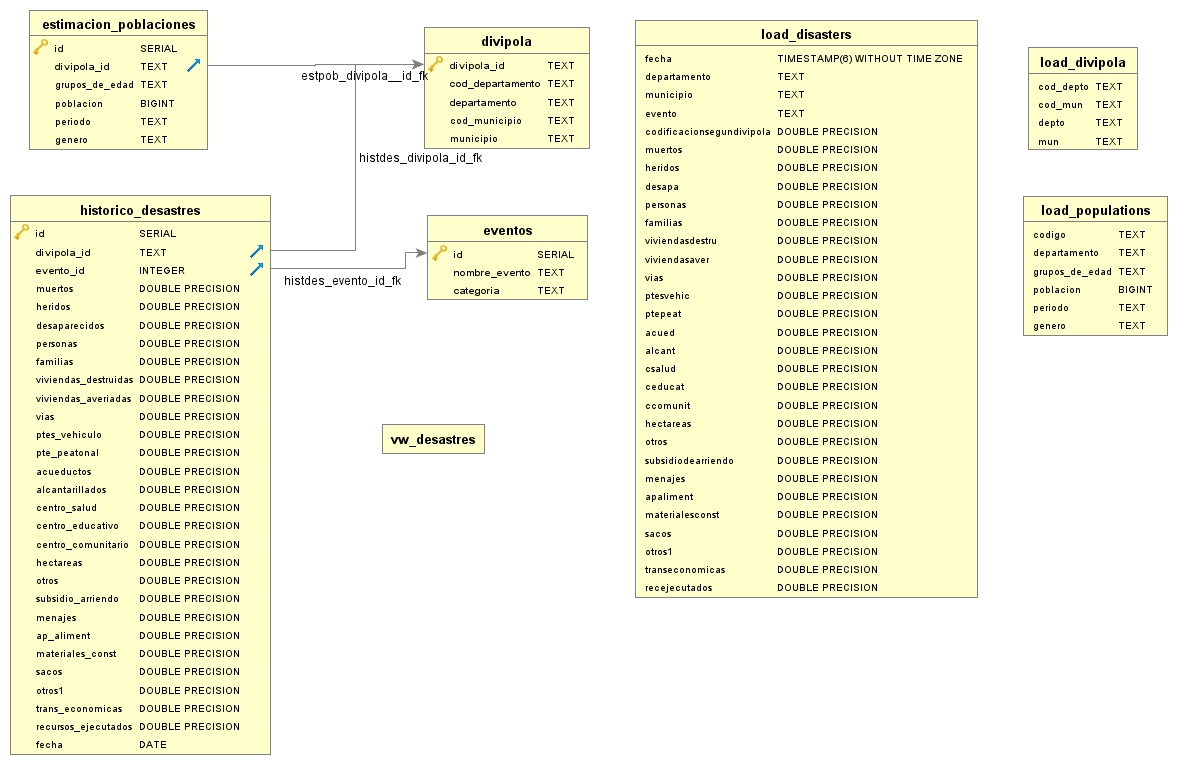
\includegraphics[width=0.95\textwidth]
{Project_Group03_ERModel}}
\caption{Entity relationship model.}
\label{fig:er_model}
\end{figure}

Figure \ref{fig:awsConnection} shows the database uploaded to AWS.

\begin{figure}[!htb]
\center{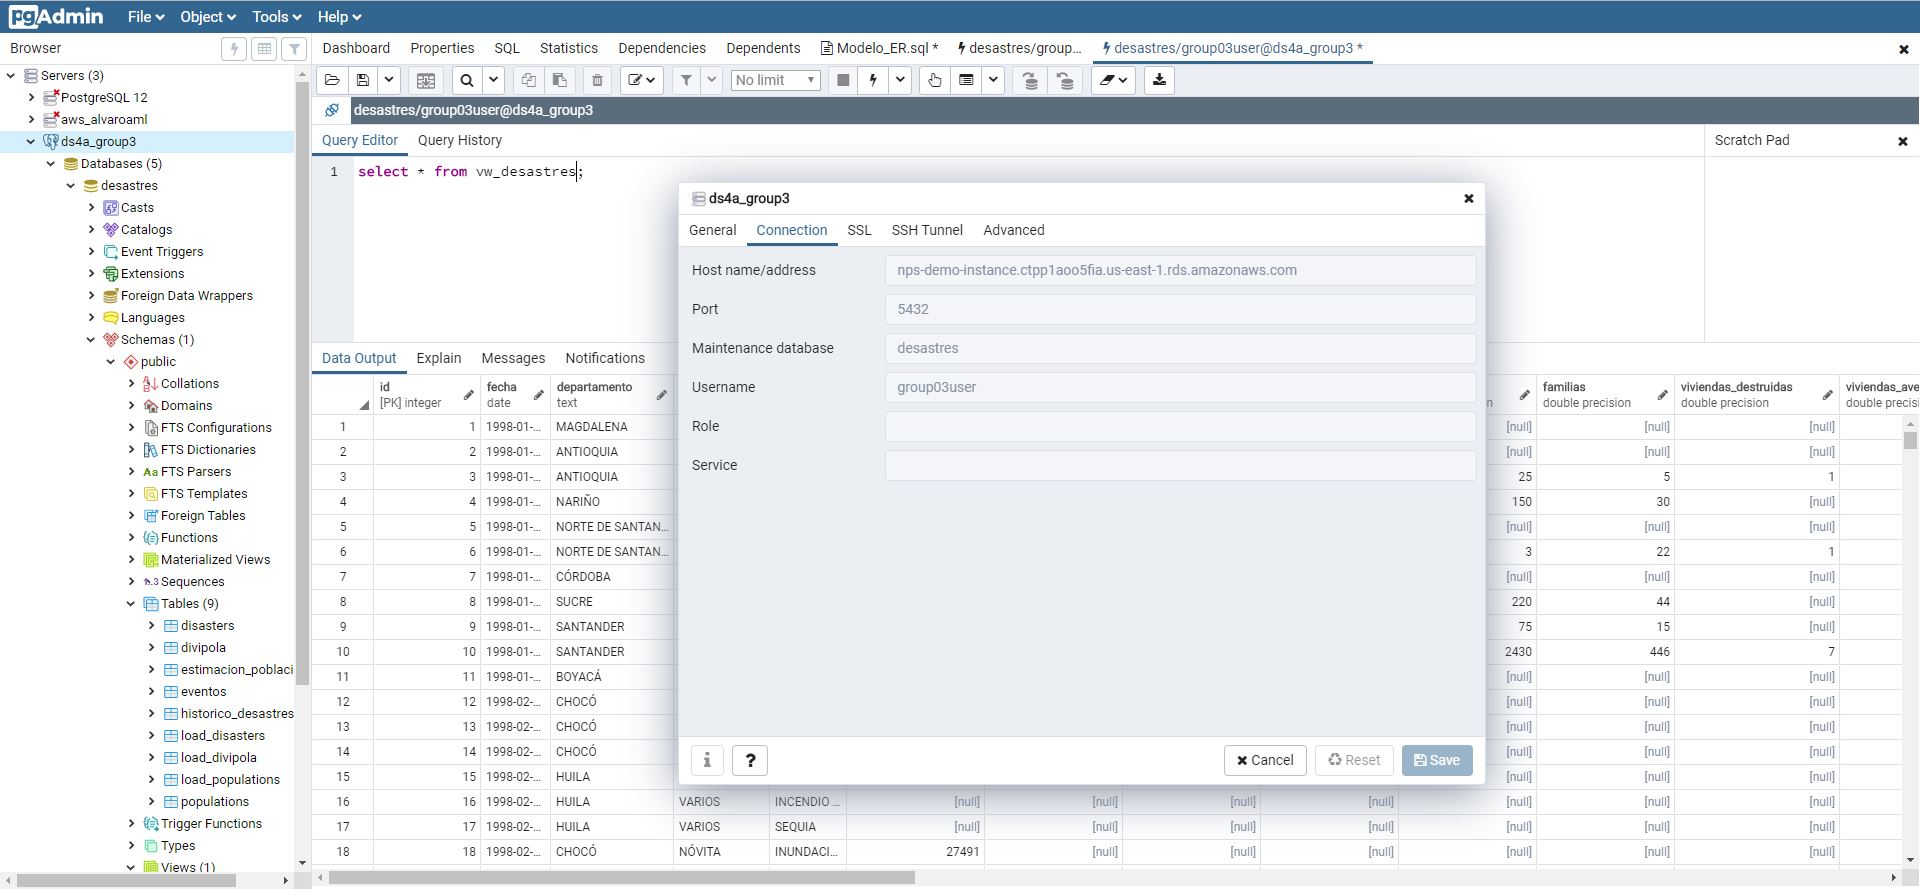
\includegraphics[width=0.95\textwidth]
{Desastres_AWS_Connection}}
\caption{AWS connection.}
\label{fig:awsConnection}
\end{figure}


Figure \ref{fig:databaseLoaded}  shows the database loaded to the AWS hosted database.

\begin{figure}[!htb]
\center{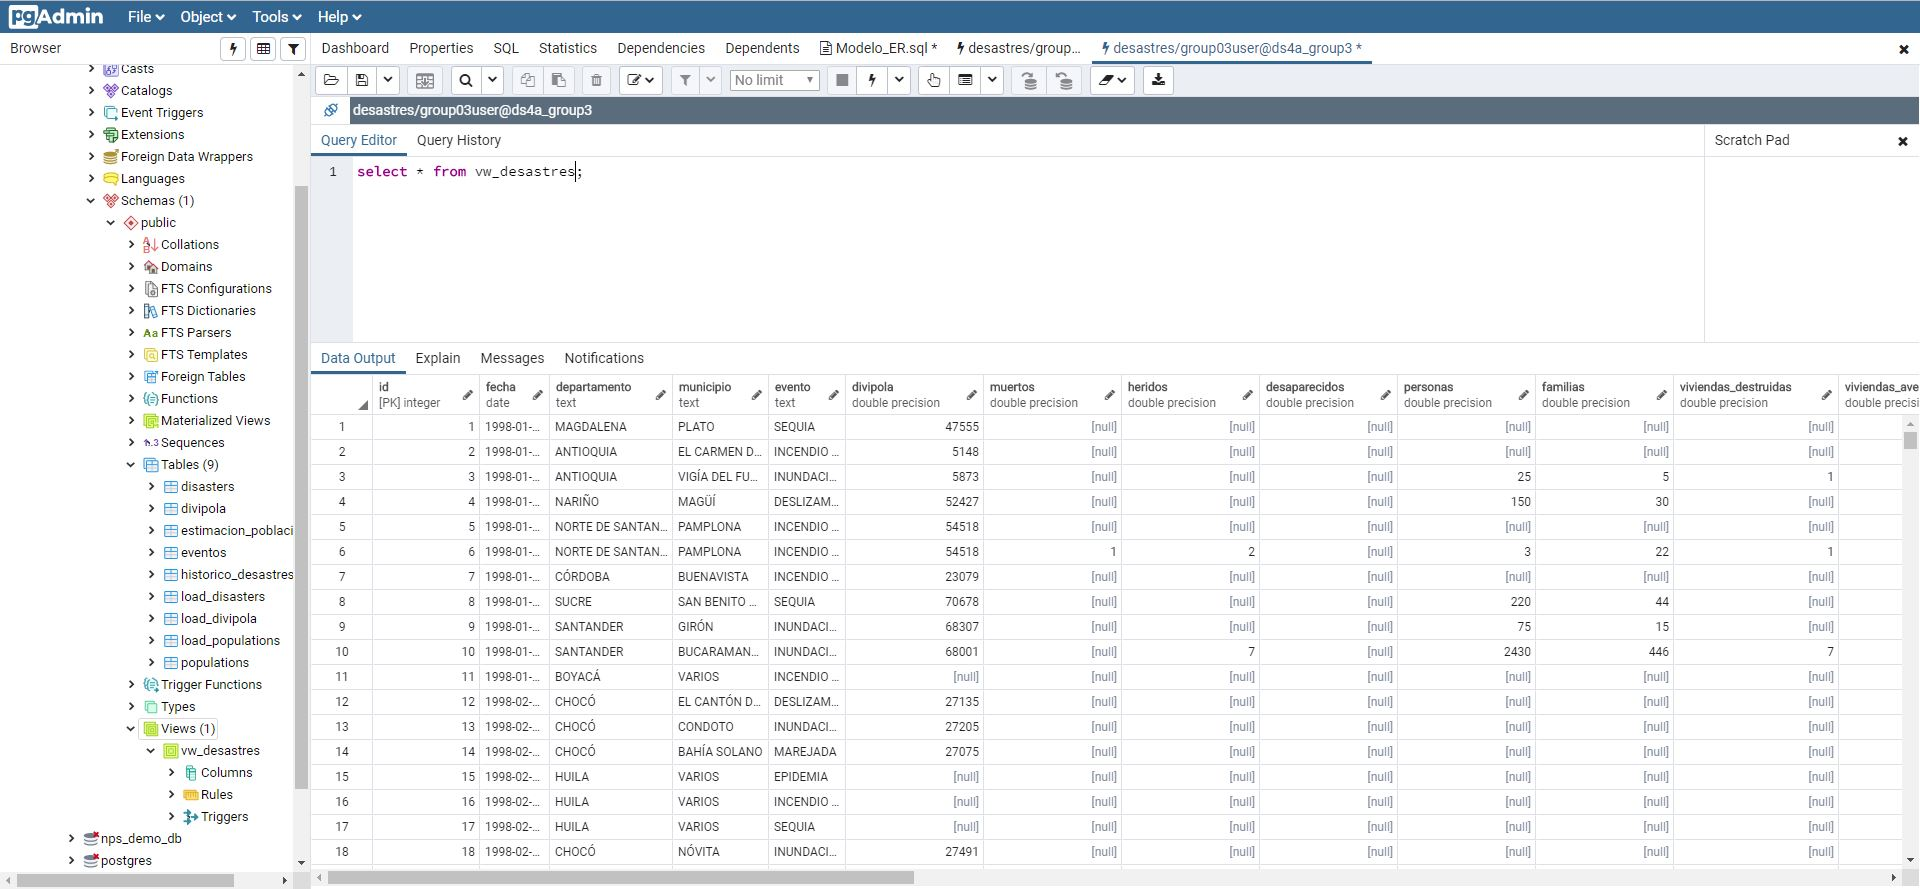
\includegraphics[width=0.95\textwidth]
{Desastres_data}}
\caption{Database loaded to AWS.}
\label{fig:databaseLoaded}
\end{figure}


The link between the front-end and the AWS-hosted databased was also stablished (see Figure \ref{fig:linkDASH_AWS}). 

\begin{figure}[!htb]
\center{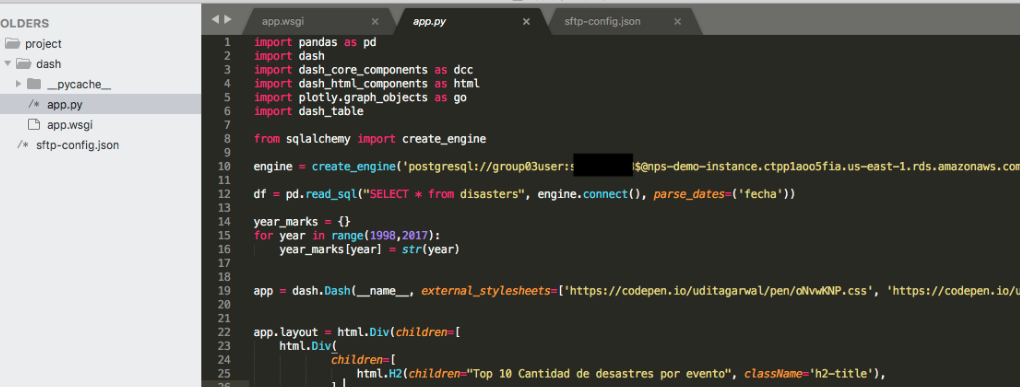
\includegraphics[width=0.95\textwidth]
{link_dash_aws}}
\caption{Link between DASH and AWS stablished}
\label{fig:linkDASH_AWS}
\end{figure}




\section{Final Thoughts}
\label{sec:Conclu}

Something we learned when building data visualizations for climate data is that you are always trying to balance simplicity of the approach with closeness to the phenomena.  Ed Hawkins, climate scientist from Reading University created the warming stripes visualization which you can see Colombia's version atop of the web application.

They show a clear picture of global warming since the 1900 in such an elegant way that they went viral and did a great service in terms of raising awareness. We took inspiration from that but decided to go into more detail in order to show how global warming affects you directly. The town you were born, the city you live.

Hopefully we accomplished some of that: Surfacing information from the past, removing friction to access current data and giving some clues about the future. This was the \textbf{challenge accepted} by 6 college educated professionals, experienced in the fields of data analytics, information management and research to put all the data together, in a way that any of us, as citizens, could make a decision, derive a conclusion or even form an opinion upon it.

Finally, to accomplish what was shown in this document, the work was divided as follows:

\begin{itemize}

\item Database AWS Computation / SQL queries: Alvaro Mu\~noz and Mario Cer\'on
\item Front End Dash App: Javier Coconubo, Jhonatan Salamanca and Jairo Ni\~no
\item Data Wrangling: Javier Coconubo, Carol Martinez, Jhonatan Salamanca and Alvaro Mu\~noz.
\item Dataset Research: Jairo Ni\~no and Carol Martinez
\item Project Management: Mario Cer\'on and Javier Coconubo
\item Documentation and reporting: Carol Martinez and Mario Cer\'on

\end{itemize}

All of the 6 members of the group collaborate in equal efforts as well. ($16,6\%$) 


\bibliographystyle{ieeetr}
\bibliography{project}

\end{document}
